\subsection{高级函数式编程}
之前的函数式编程当中,提到了map函数,用于对数据进行处理,比如下面这种:
\begin{code-block}{rust}
let sum: u32 = c1
    .zip(c2.skip(10))
    .map(|(a, b)| a * b)
    .filter(|x| x % 3 == 0)
    .sum();
\end{code-block}

但是,实际使用当中,map还有更加广泛的用途,比如,在特定的情况下,替换match操作,
使得代码更加简单和精炼。比如,在使用match处理Option这种数据类型时,由于Option的
取值范围为Some和None,而map函数对于Option类型的处理,也恰好就是返回Some和None,
因此,可以直接使用map函数对这种Some对Some,None对None的简单映射关系进行处理,
多个不同的map进行组合,形成链式调用,相比而言,比match操作会更加简练:
\begin{code-block}{rust}
#[derive(Debug)]
enum Food {
    Apple,
    Potato,
}

#[derive(Debug)]
struct Peeled(Food);
#[derive(Debug)]
struct Chopped(Food);
#[derive(Debug)]
struct Cooked(Food);

// 常见的处理方法,使用match进行处理,并且返回一个Option
fn peel(food: Option<Food>) -> Option<Peeled> {
    match food {
        Some(food) => Some(Peeled(food)),
        None => None,
    }
}

// 使用map函数进行Option的简单映射
fn process(food: Option<Food>) -> Option<Cooked> {
    food.map(|f| Peeled(f))
        .map(|Peeled(f)| Chopped(f))
        .map(|Chopped(f)| Cooked(f))
}
\end{code-block}

然而,如果返回类型Option需要作为map函数的参数,输入到另外一个闭包或者函数当中,
则有可能出现Option<Option<T>>的结果出现,并不利于结果的解析,此时,则需要采用
and\_then进行处理,比如下方的代码:
\begin{code-block}{rust}
enum Food {
    CordonBleu,
    Steak,
    Sushi,
}

fn have_ingredients(food: Food) -> Option<Food> {
    match food {
        Food1::Sushi => None,
        _ => Some(food),
    }
}

fn have_recipe(food: Food) -> Option<Food> {
    match food {
        Food1::CordonBleu => None,
        _ => Some(food),
    }
}

// 通过map函数将上述2个函数进行连接起来,have_recipe当作一个闭包使用
// 但是,结果将变更为Option<Option<T>>
fn cookable_v1(food: Food) -> Option<Option<Food>> {
    have_ingredients(food).map(|res| have_recipe(res))
}

// 通过and_then将2个函数连接起来,形成链式调用
// have_ingredients返回的是一个Option,and_then会将其进行拆包
// 如果Option是None,则直接返回None;但是,如果是Some<T>,and_then则会将其
// 进行拆包,返回为T,而不是Some<T>
fn cookable_v2(food: Food) -> Option<Food> {
    have_ingredients(food).and_then(have_recipe)
}
\end{code-block}

Result和Option类似,但实质上,Option是Result的一个特化版本,可以将其简单的看作:
\begin{code-block}{rust}
type Option<T> = Result<T, ()>
\end{code-block}

因此,Option的map,and\_then等函数(算子)同样可以作用于Result上,比如下面的例子:
\begin{code-block}{rust}
use std::num::ParseIntError;

// 使用普通的match模式
fn multiply_v1(first_number_str: &str, second_number_str: &str) -> Result<i32, ParseIntError> {
    match first_number_str.parse::<i32>() {
        Ok(first_number)  => {
            match second_number_str.parse::<i32>() {
                Ok(second_number)  => {
                    Ok(first_number * second_number)
                },
                Err(e) => Err(e),
            }
        },
        Err(e) => Err(e),
    }
}

// 使用map与and_then模式
fn multiply_v2(first_number_str: &str, second_number_str: &str) -> Result<i32, ParseIntError> {
    // and_then将Result<T, E>拆分,如果是Err,直接返回,如果是T,即Ok(T)
    // 则进行解析为T
    first_number_str.parse::<i32>().and_then(|first_number| {
        second_number_str.parse::<i32>().map(|second_number| first_number * second_number)
    })
}
\end{code-block}

同样的,Result也可以使用别名系统,比如常见的io::Result,实际上就是Result的一个
别名特化版本:
\begin{code-block}{rust}
type Result<T> = Result<T, Error>;
\end{code-block}
因此,同样可以在代码当中使用Result的别名,对代码进行简化:
\begin{code-block}{rust}
use std::num::ParseIntError;

type AliasedResult<T> = Result<T, ParseIntError>;

fn multiply(first_number_str: &str, second_number_str: &str) -> AliasedResult<i32> {
    first_number_str.parse::<i32>().and_then(|first_number| {
        second_number_str
            .parse::<i32>()
            .map(|second_number| first_number * second_number)
    })
}

fn print(result: AliasedResult<i32>) {
    match result {
        Ok(n) => println!("n is {}", n),
        Err(e) => println!("Error: {}", e),
    }
}

fn main() {
    print(multiply("10", "2"));
    print(multiply("t", "2"));
}
\end{code-block}

由于Option和Result的特殊性,在一些特定的场合,尤其是处理错误的时候,常见的做法就是
混合Option和Result,进行混合类型的错误处理:
\begin{code-block}{rust}
use std::num::ParseIntError;

fn double_first(vec: Vec<&str>) -> Option<Result<i32, ParseIntError>> {
    // map返回Option,使用map包裹parse函数可能带来的错误信息(Result)
    vec.first().map(|first| first.parse::<i32>().map(|n| 2 * n))
}

fn double_first_v2(vec: Vec<&str>) -> Result<Option<i32>, ParseIntError> {
    let opt = vec.first().map(|first| first.parse::<i32>().map(|n| 2 * n));

    // map_or返回Result,其中,Ok子句处理opt为None的情况
    // r则处理opt为Some和Err的情况
    opt.map_or(Ok(None), |r| {
        println!("The r is error {:?}", r);
        r.map(Some)
    })
}

fn main() {
    let empty2 = vec![];

    match double_first_v2(empty2) {
        Ok(Some(x)) => println!("The result is {}", x),
        Err(e) => println!("Error is {:?}", e),
        Ok(None) => println!("None is in result"),
    }
}
\end{code-block}

\subsection{自定义错误}
Rust的错误是可以进行自行定义的,只需要实现一个Error Trait即可。Error Trait的定义
如下:
\begin{code-block}{rust}
pub trait Error: Debug + Display {
    fn source(&self) -> Option<&(dyn Error + 'static)> { ... }
    fn backtrace(&self) -> Option<&Backtrace> { ... }
    fn description(&self) -> &str { ... }
    fn cause(&self) -> Option<&dyn Error> { ... }
}
\end{code-block}
其中:
\begin{itemize}
  \item source是必须实现的函数,并且对应的错误必须实现Debug和Display Trait
  \item backtrace是只能在nightly分支当中实现的函数
  \item description被废弃,使用Display Trait或者to\_string(ToString Trait)替代
  \item cause同样被废弃,被source所取代
\end{itemize}

一个简单的例子如下:
\begin{code-block}{rust}
use std::error::Error;
use std::fmt;

// 定义自定义错误结构体
// 实现Debug Trait
#[derive(Debug)]
struct SuperError {
    msg: String,
}

// 实现Display Trait
impl fmt::Display for SuperError {
    fn fmt(&self, f: &mut fmt::Formatter) -> fmt::Result {
        write!(f, "Super Error: {}", self.msg)
    }
}

// 实现Error Trait
impl Error for SuperError {
    fn source(&self) -> Option<&(dyn Error + 'static)> {
        Some(self)
    }
}

impl SuperError {
    fn new(err: &str) -> SuperError {
        SuperError {
            msg: err.to_string(),
        }
    }
}

fn err_test() -> Result<(), SuperError> {
    Err(SuperError::new("first error"))
}

fn main() {
    match err_test() {
        // Err(SuperError{msg: e}) => println!("{}", e),
        Err(e) => println!("{}", e),
        _ => println!("no error"),
    }
}
\end{code-block}

错误和自定义错误解决的是对于错误的定义,以及对应错误的处理方式,但是,在实际的生产
使用当中,错误可能是普遍存在的,而我们需要的数据可能并不包含错误信息,而是需要
将错误从正确的结果当中剔除,比如:
\begin{code-block}{rust}
fn main() {
    let strings = vec!["tofu", "93", "18"];
    let possible_numbers: Vec<_> = strings.into_iter().map(|s| s.parse::<i32>()).collect();
    println!("Results: {:?}", possible_numbers);
}
\end{code-block}
我们的本意是将Vec当中的字符串全部格式化为数值,但是,实际的结果当中,却把包含的
错误也一同包含进来了,需要想办法将错误信息过滤掉:
\begin{code-block}{rust}
fn main() {
    let strings = vec!["tofu", "93", "18"];
    let numbers: Vec<_> = strings
        .into_iter()
        .map(|s| s.parse::<i32>())
        // filter_map进行过滤,只保留结果为ok的数据
        .filter_map(Result::ok)
        .collect();
    println!("Results: {:?}", numbers);
}
\end{code-block}

Result实现了FromIter,因此结果的向量(Vec<Result<T, E>>)可以被转换成结果包裹着
向量(Result<Vec<T>, E>)。一旦找到一个Result::Err,遍历就被终止,即满足另外一种
需求:只要任何一个错误发生,就中断当前的操作:
\begin{code-block}{rust}
fn main() {
    let strings = vec!["tofu", "93", "18"];
    // 注意numbers不再是Vec<_>,而是通过FromIter转换成了Result
    // 转换过程一旦失败,就会出现错误,中断当前的执行流程
    let numbers: Result<Vec<_>, _> = strings.into_iter().map(|s| s.parse::<i32>()).collect();
    println!("Results: {:?}", numbers);
}
\end{code-block}

但是,有的时候,我们也存在另外一种需求:将执行的正确和错误结果分类存放,以待后续
操作,此时则需要使用partition函数,对结果进行区分:
\begin{code-block}{rust}
fn main() {
    let strings = vec!["tofu", "93", "18"];
    let (numbers, errors): (Vec<_>, Vec<_>) = strings
        .into_iter()
        .map(|s| s.parse::<i32>())
        // 使用partition函数进行区分
        .partition(Result::is_ok);
    println!("Numbers: {:?}", numbers);
    println!("Errors: {:?}", errors);

    // 对后续的结果进行解构
    let numbers: Vec<_> = numbers.into_iter().map(Result::unwrap).collect();
    let errors: Vec<_> = errors.into_iter().map(Result::unwrap_err).collect();
    println!("Numbers: {:?}", numbers);
    println!("Errors: {:?}", errors);
}
\end{code-block}

\section{死灵书与实践}

\subsection{随机数实践}
Rust的随机数模块并不包含在标准库当中,需要使用rand这个crate,其基本的使用如下:
\begin{code-block}{rust}
use rand::distributions::{Distribution, Uniform};
use rand::seq::IteratorRandom;
use rand::Rng;

fn main() {
    let mut rng = rand::thread_rng();
    // 生成随机数
    info!("The float64 rand number is {}", rng.gen::<f64>());
    info!("The u32 rand number is {}", rng.gen::<u32>());
    info!("The i32 rand number is {}", rng.gen::<i32>());
    info!("The u8 rand number is {}", rng.gen::<u8>());
    // 从指定区间生成随机数
    info!("The range rand number is {}", rng.gen_range(0..100));
    info!(
        "The range rand float number is {}",
        rng.gen_range(10.0..50.0)
    );
    // 从[0, 5]生成随机数
    info!("The range rand number is {}", rng.gen_range(0..=5));

    // 定义[1, 7)的均匀分布
    let die = Uniform::from(1..7);
    // 从该分布当中生成采样
    let throw = die.sample(&mut rng);
    info!("The sample of uniform is {:>width$}", throw, width = 5);

    // 生成多个随机数
    let tuple: (u8, u8, u8) = rng.gen();
    info!("The tuple of random is {:?}", tuple);
    // 生成随机数组
    let array: [u8; 6] = rng.gen();
    info!("The array of random is {:?}", array);
    let mut exsit_array: [u8; 5] = [1, 2, 34, 5, 6];
    // 使用随机数填充已存在的数组
    rng.fill(&mut exsit_array);
    info!("The array of random is {:?}", exsit_array);

    // 从均匀分布当中随机采样3个数据
    // 得到的结果可能出现重复的情况
    let samples: Vec<u8> = (&mut rng).sample_iter(die).take(3).collect();
    info!("The samples of sample range 1..7 is {:?}", samples);

    let v = vec![1, 2, 3, 4, 5];
    // 从vec当中采样4个数据,得到的结果不会重复
    let sample = v.iter().choose_multiple(&mut rng, 4);
    info!("The samples of sample range 1..5 is {:?}", sample);
    let sample: Vec<u8> = (1..=10).choose_multiple(&mut rng, 4);
    info!("The samples of sample range 1..10 is {:?}", sample);
}
\end{code-block}

Rust的rand crate不仅可以生成随机数,也可以生成自定义的随机数据,比如:
\begin{code-block}{rust}
use rand::distributions::{Distribution, Standard, Uniform};
use rand::seq::IteratorRandom;
use rand::Rng;

struct Point {
    x: u8,
    y: u8,
}

impl fmt::Display for Point {
    fn fmt(&self, f: &mut fmt::Formatter) -> fmt::Result {
        write!(f, "x: {}, y: {}", self.x, self.y)
    }
}

// 在 Point 类型之上,对Standard实现Distribution trait,使得Point可以被gen函数随机生成
impl Distribution<Point> for Standard {
    // 默认的实现方法
    fn sample<R: Rng + ?Sized>(&self, rng: &mut R) -> Point {
        let (rand_x, rand_y) = rng.gen();
        Point {
            x: rand_x,
            y: rand_y,
        }
    }
}

fn main() {
    let mut rng = rand::thread_rng();
    let rand_point = rng.gen::<Point>();
    info!("The rand_point is {}", rand_point);
}
\end{code-block}

同样的,可以生成随机的字符串:
\begin{code-block}{rust}
use rand::distributions::{Alphanumeric, Distribution, Standard, Uniform};
use rand::seq::IteratorRandom;
use rand::Rng;

fn main() {
    let mut rng = rand::thread_rng();
    let rand_string: String = (&mut rng)
        // 从a-z,A-Z以及0-9当中进行选择
        .sample_iter(&Alphanumeric)
        // 获取其中的10个元素
        .take(10)
        // 默认的结果是char类型,需要继续转换成String
        .map(char::from)
        .collect();
    info!("The rand_string is {}", rand_string);
}
\end{code-block}

如果默认的字符集不满足要求,还可以自定义字符集,比如下面的示例:
\begin{code-block}{rust}
use rand::distributions::{Alphanumeric, Distribution, Standard, Uniform};
use rand::seq::IteratorRandom;
use rand::Rng;
const CHARSET: &[u8] = b"ABCDEFGHIJKLMNOPQRSTUVWXYZ\
    abcdefghijklmnopqrstuvwxyz\
    0123456789)(*&^%$#@!~";
const PASSWORD_LEN: usize = 10;

fn main() {
    let mut rng = rand::thread_rng();
    let password: String = (0..PASSWORD_LEN)
        .map(|_| {
            let idx = rng.gen_range(0..CHARSET.len());
            CHARSET[idx] as char
        })
        .collect();
    info!("The password is {}", password);

    // 也可以更换成之前的采样函数,看起来更为精炼
    let passwd: String = CHARSET
        .choose_multiple(&mut rng, 10)
        .map(|r| *r as char)
        .collect();
    info!("The password is {}", passwd);
}
\end{code-block}

同样的,针对自定义的数据类型,同样可以采用采样方法,进行随机数据的提取:
\begin{code-block}{rust}
use rand::distributions::{Alphanumeric, Distribution, Standard, Uniform};
use rand::seq::IteratorRandom;
use rand::Rng;

#[derive(Debug)]
struct Person {
    name: String,
    age: u8,
}

fn main() {
    let mut rng = rand::thread_rng();
    let persons = vec![
        Person {
            name: "lucifer".to_string(),
            age: 18,
        },
        Person {
            name: "titans".to_string(),
            age: 19,
        },
        Person {
            name: "garuda".to_string(),
            age: 36,
        },
    ];

    // 从person的vec当中,随机抽取2个元素
    let rand_person: Vec<_> = persons.choose_multiple(&mut rng, 2).collect();
    info!("The rand person is {:?}", rand_person);
}
\end{code-block}

\subsection{类型再论}
Rust的类型比较多,char,字符串,整数,浮点数等等。这些基础类型和其他语言比较类似,
但是也包含了自己的特点:比如,char类型占据4个字节,可以存放任何一个unicode字符;
对于ASCII字符,只需要一个字节即可,而一个字节的数据,则可以放在u8类型的数据当中,
因此,对于ASCII类型的字符串/字符数组,可以使用u8类型(即单字节)的数组进行存放,
这样,占用的资源空间会比char的数组小:
\begin{code-block}{rust}
fn main() {
    // 字符串前面的b,表示将对应的字面量存放在u8类型当中
    let s: &[u8] = b"hello";
    info!("{:?}", s);
}
\end{code-block}
同时,Rust支持的整数类型比较广泛,包括8bit,16bit,32bit,64bit,最大可以支持到
128bit;而特殊的isize和usize,则是和平台相关。如果平台是32位的,则isize和usize为
32位,如果是64位,则其数据宽度为64位。

整个Rust的类型当中,只有空类型占据的空间是最小的,都是0。Rust的空类型包括单元类型
(unit,即空元组)以及空结构体:
\begin{code-block}{rust}
// empty是空元组类型
let empty : () = ();

// 空结构体
struct Empty();
\end{code-block}
为了查看类型所占用的空间,可以使用size\_of函数进行查看:
\begin{code-block}{rust}
use std::mem;

struct Empty();
fn main() {
    info!("The Empty struct size is {}", mem::size_of::<Empty>());
    // 查看空元组所占据的内存大小
    info!("The none tuple size is {}", mem::size_of::<()>());
}
\end{code-block}

在Rust当中,浮点类型是非常特殊的数据类型。浮点类型当中,存在一个特殊的值:NaN,
即非法的浮点数值,因为该数据的存在,浮点数不具备全序关系(total order)。所谓的
全序,偏序,Rust当中的定义如下:对于集合X当中的元素a,b,c
\begin{itemize}
  \item 如果a<b,则!(a>b)一定成立;反之,如果a>b,则!(a<b)一定成立,即反对称性
  \item 如果a<b,b<c,则a<c,即传递性
  \item 对于X当中的所有元素,都存在a<b,或者a>b,或者a==b,三者必居其一,即完全性
\end{itemize}
如果X集合只满足前面2条,则称之为偏序;具备上述所有特征,则为全序。由于浮点数的NaN
不满足上述第3条规则,因此,Rust的浮点数属于偏序,而非全序,这回导致一个问题:浮点
数无法排序——非NaN的数值无法与NaN进行比较:
\begin{code-block}{rust}
let nan = std::f32::NAN;
let x = 0.4f32;
// 下列结果全部为false
info!("{}", nan > x);
info!("{}", nan < x);
info!("{}", nan == x);
\end{code-block}
为此,Rust设计了2个Trait表示全序与偏序:\mintinline[breaklines=true,breakanywhere,breaksymbolleft=,breakanywheresymbolpre=,]{rust}{std::cmp::Ord}(全序)以及
\mintinline[breaklines=true,breakanywhere,breaksymbolleft=,breakanywheresymbolpre=,]{rust}{std::cmd::PartialOrd}(偏序)。
PartialOrd这个Trait的partial\_cmp方法返回的是Option<Ordering>,而Ord返回的却是
Ordering。Rust的f32和f64都只实现了PartialOrd,因此,浮点类型无法进行排序,也同样无法
求取最值,如下列代码,则是无法运行的:
\begin{code-block}{rust}
let f_vec = vec![1f32, 2.0, 4.0, 0.0, -1.2];
let bigest_f = f_vec.iter().max();
\end{code-block}
对上诉代码进行编译,会直接提示如下类似的错误:
\begin{figure}[H]
  \centering
  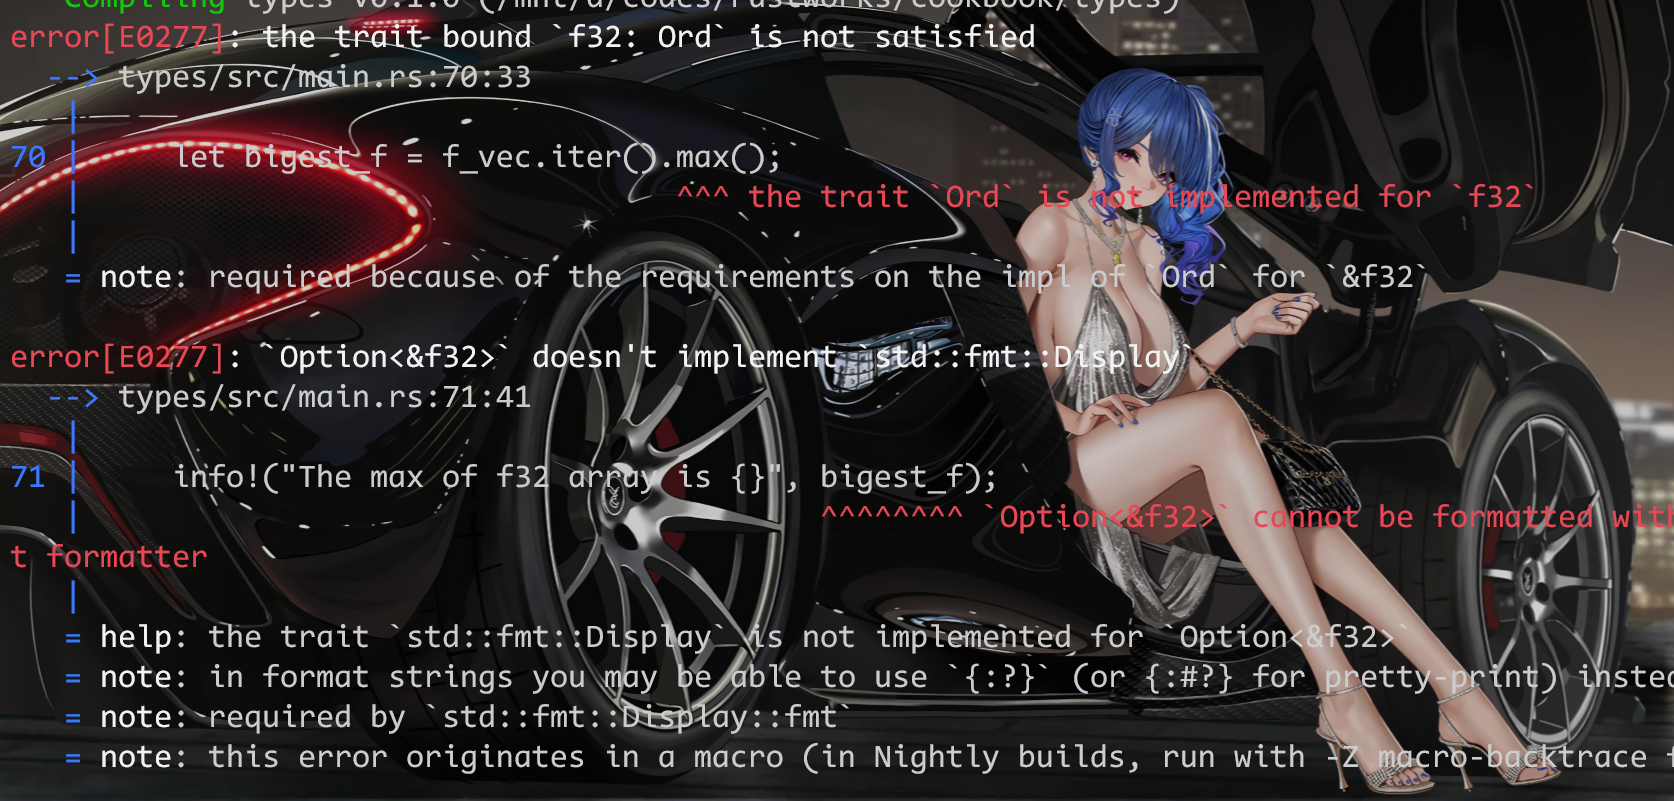
\includegraphics[scale=0.2]{rust_float_cmp_error.png}
  \caption{浮点数的最值错误求解}
  \label{fig:rust_float_cmp_error}
\end{figure}
浮点数的排序只能通过partial\_cmp(比较相等关系)进行变换处理,如下方代码:
\begin{code-block}{rust}
let mut f_vec = vec![1f32, 2.0, 4.0, 0.0, -1.2];
// 升序排列
f_vec.sort_by(|first, second| first.partial_cmp(second).unwrap());
// 获取排序后的最后一位
let max = f_vec.last().unwrap();
// 或者如下进行
// let max = f_vec.as_slice().last().unwrap();
// 降序排列
f_vec.sort_by(|first, second| second.partial_cmp(first).unwrap());
\end{code-block}

作为常用数据类型之一,Rust的数组也存在自己的特点,比如同类型的数组之间可以相互赋值:
\begin{code-block}{rust}
let mut array: [u32; 4] = [1, 23, 4, 5];
let array_copy: [u32; 4] = [5, 6, 7, 8];
array = array_copy;
\end{code-block}
支持数组之间的直接比较,只是数组当中的元素本身就可以进行比较才行:
\begin{code-block}{rust}
let array: [u32; 4] = [1, 23, 4, 5];
let array_copy: [u32; 4] = [5, 6, 7, 8];
info!("{:?}", array < array_copy);
\end{code-block}

Rust当中的函数也可以称之为类型的一种,并且,每个函数都有自己单独的类型,函数的类型
是fn。但是,函数的参数列表会影响fn类型的判断和表达,比如下面的例子:
\begin{code-block}{rust}
fn add_tuple(t: (u32, u32)) -> u32 {
    t.0 + t.1
}

fn add_two((x, y): (u32, u32)) -> u32 {
    x + y
}

fn add_normal(x: u32, y: u32) -> u32 {
    x + y
}

\end{code-block}
实际上,add\_tuple和add\_two这2个函数被fn类型识别成为具有相同签名的类型,因此,
在理论上,我们可以使用同一个变量,接收这2个函数的指针:
\begin{code-block}{rust}
fn main() {
    let mut func = add_tuple;
    func = add_two;
    ...
}
\end{code-block}
但是,上述代码却是错误的:虽然签名相同,但是,类型不同:
\begin{figure}[H]
  \centering
  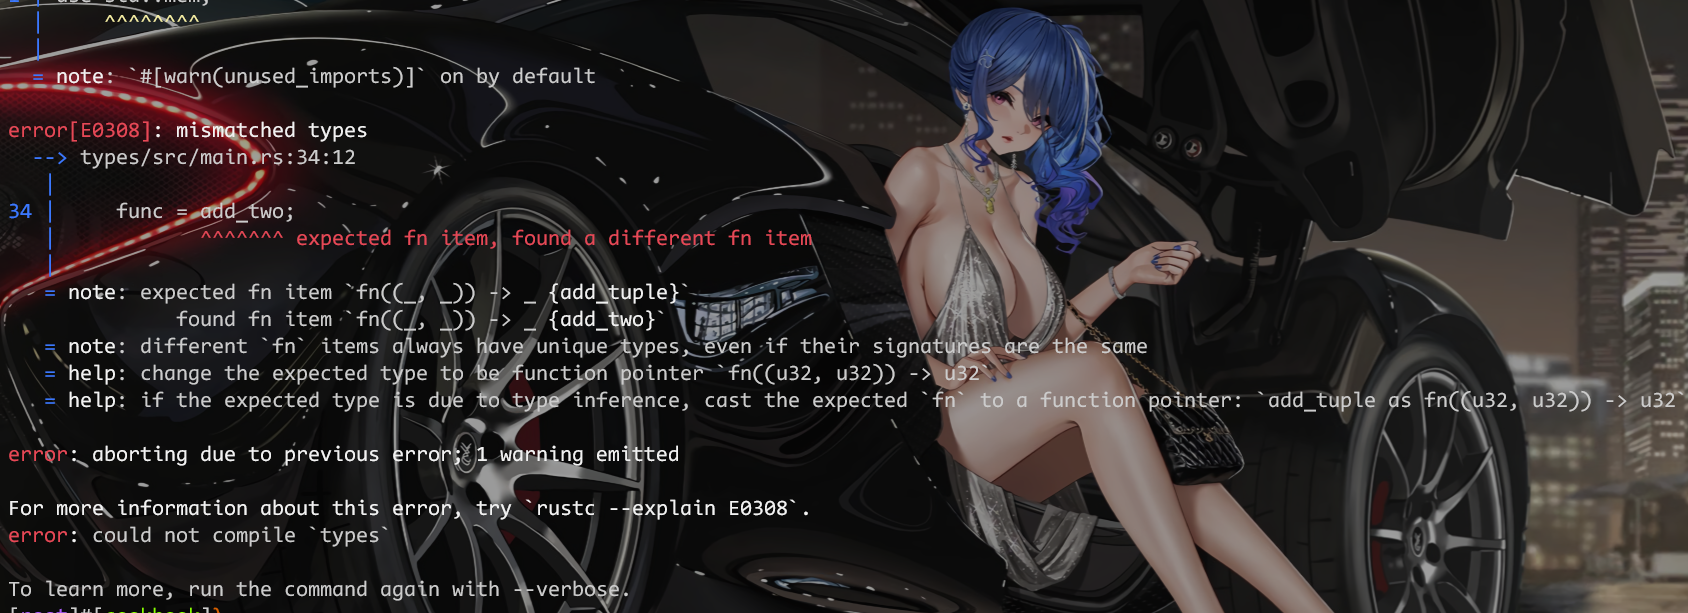
\includegraphics[width=\linewidth]{rust_func_type.png}
  \caption{相同签名的不同函数类型}
  \label{fig:rust_func_type}
\end{figure}
解决方法,则是将其转换成通用的fn类型:
\begin{code-block}{rust}
fn main() {
    // 显示指定func的类型
    let mut func: fn((u32, u32)) -> u32 = add_tuple;
    // 使用as进行类型的转换
    // let mut func = add_tuple as fn((u32, u32)) -> u32;
    func = add_two;
    ...
}
\end{code-block}
但是,需要注意,add\_normal的功能看上去和前面两个函数的功能相同,但是,他们的
函数签名完全不同,因此,不能将其转换成func。

函数是Rust的头等公民,可以在函数/方法当中定义函数,也可以在函数/方法当中定义结构
体,甚至于定义结构体的方法和实现,以及静态变量,常量等:
\begin{code-block}{rust}
fn func_as_first(x: u32, y: u32) -> (u32, u32) {
    struct Point {
        x: u32,
        y: u32,
    };

    impl Point {
        fn area(&self) -> u32 {
            self.x * self.y
        }
        fn cycle(&self) -> u32 {
            self.x + self.y
        }
    };

    let p = Point { x: x, y: y };
    (p.area(), p.cycle())
}
\end{code-block}

常规的函数类型,都会存在返回值,这些返回值要么是特定的类型,要么就是(),即类似
C/C++的返回void。如果需要什么都不返回,则可以使用!,这种函数称之为发散函数,比如
在处理panic时,有时就需要使用发散函数:
\begin{code-block}{rust}
fn diverges() -> ! {
    panic!("This function never returns!");
}
\end{code-block}
Panic操作会直接导致软件栈展开,因此,后续的操作都不会执行,其返回的就是一个!。
发散函数的最大特点,就是可以被转换成任意一个类型,虽然执行的时候最终还是会崩溃,
如下:
\begin{code-block}{rust}
let x : i32 = diverges();
let y : String = diverges();
\end{code-block}
但是,发散函数最大的作用,在于解决编译器的类型检查:
\begin{code-block}{rust}
let p = if x {
    panic!("error");
} else {
    100
};
\end{code-block}
对于let-if而言,if-else的每个分支都必须是相同的数据类型,通过发散函数的任意类型
转换特性即!与任何类型兼容,所以上述代码才能编译通过。

所有的Rust变量,函数都是类型的一种,都可以通过一定的手段和方式,获得类型的具体信息。
常见的方式有两种,一种是使用错误信息进行推断,一种则是使用标准库函数进行获得。

通过构造一个特殊的函数,然后调用该函数,则可以获得相关的类型信息:
\begin{code-block}{rust}
// 接收一个unit参数
fn type_id(_: ()) {}

fn main() {
    let ref i = 5;
    type_id(i);
}
\end{code-block}

而另外的方式,则是使用标准库函数,不过,这个标准库函数在Rust的默认stable分支当中
是不可用的,需要在nightly分支当中进行编译使用,并且,还需要启用一些特性:
\begin{code-block}{rust}
#![feature(core_intrinsics)]
use std;

// 使用泛型参数进行不同类型的数据接收
fn print_type<T>(_arg: &T) {
    println!(
        "The type name of arg is {}",
        std::intrinsics::type_name::<T>()
    );
}

fn main() {
    let ref x = 5;
    print_type(&x);
}
\end{code-block}
编译上述代码时,则需要对编译指令进行部分的调整:
\mintinline[breaklines=true,breakanywhere,breaksymbolleft=,breakanywheresymbolpre=,]{bash}{cargo +nightly build},
然后即可实现对参数类型的打印输出。

在Rust当中,与Python不同,函数/方法并不存在默认参数,但是,结构体当中的字段,却可以
有默认值,只是,这个默认值的实现,必须和Default Trait相结合,如下:
\begin{code-block}{rust}
struct ColoredString {
    input: String,
    fg_color: String,
    bg_color: String,
}

impl Default for ColoredString {
    fn default() -> Self {
        ColoredString {
            input: String::default(),
            fg_color: String::default(),
            bg_color: String::default(),
        }
    }
}

fn main() {
    let color = ColoredString::default();
}
\end{code-block}
从上述代码当中可以看出,实际上,并不是Rust的结构体字段赋予了初始值,而是通过一个
名为default的方法,构造一个我们认为应该具有默认值的结构体。在Rust当中,常用的基本
数据类型都实现了Default Trait,可以直接使用对应的default方法。

\subsection{Trait类型与泛型再论}
关于类型,Trait也是比较重要的一个话题。在之前的示例当中,Trait全部是在具体的类型
上实现的,但是,Trait本身也可以在智能指针(Box)上实现,比如:
\begin{code-block}{rust}
trait Shape {
    fn area(self: Box<Self>) -> f64;
}
struct Circle {
    radius: f64,
}
impl Shape for Circle {
    fn area(self: Box<Self>) -> f64 {
        PI * self.radius * self.radius
    }
}
fn main() {
    let c = Box::new(Circle { radius: 4f64 });
    info!("{}", c.area());
    // 由于trait实现是在智能指针box上,因此,下面的使用是错误的
    // let c = Circle { radius: 4f64 }
    // c.area()
}
\end{code-block}
甚至在Trait上实现Trait,比如下方:
\begin{code-block}{rust}
trait Shape {
    fn area(&self) -> f64;
}
trait Round {
    fn get_radius(&self) -> f64;
}
struct Circle {
    radius: f64,
}
impl Round for Circle {
    fn get_radius(&self) -> f64 {
        self.radius
    }
}
impl Shape for dyn Round {
    fn area(&self) -> f64 {
        let radius = self.get_radius();
        PI * radius * radius
    }
}
\end{code-block}
Shape是一个Trait,Round同样也是一个Trait,Circle实现了Round,Round实现了Shape,
但是,由于Round本身是一个Trait,拥有不确定性,因此,在实现Shape的时候,需要添加
dyn关键字,提示这个Round不是普通的类型,而是一个Trait。上述代码当中,Circle间接
的实现了Shape,但是,Circle的类型无法直接使用Shape的方法,只能通过智能指针的方
式,将Circle转换成Round的类型,再进行使用,如下:
\begin{code-block}{rust}
fn main() {
    let c: Box<dyn Round> = Box::new(Circle { radius: 4f64 });
    info!("{}", c.area());
}
\end{code-block}
如果再把这个例子改得复杂一些,让Circle和Sphere同时实现Round,则我们可以使用Round
指针计算2个不同类型数据的结果:
\begin{code-block}{rust}
trait Shape {
    fn area(&self) -> f64;
}
trait Round {
    fn calc(&self) -> f64;
}
struct Circle {
    radius: f64,
}
impl Round for Circle {
    fn calc(&self) -> f64 {
        PI * self.radius * self.radius
    }
}
struct Sphere {
    radius: f64,
}
impl Round for Sphere {
    fn calc(&self) -> f64 {
        4f64 * PI * self.radius * self.radius
    }
}
impl Shape for dyn Round {
    fn area(&self) -> f64 {
        self.calc()
    }
}
fn main() {
    let circle: Box<dyn Round> = Box::new(Circle { radius: 4f64 });
    info!("The Circle area is {}", circle.area());
    let sphere: Box<dyn Round> = Box::new(Sphere { radius: 4f64 });
    info!("The Sphere area is {}", sphere.area());
}
\end{code-block}

Trait不仅仅用于实现类型,约束类型,还可以用于为其他现有的数据类型添加方法/函数,
比如:
\begin{code-block}{rust}
impl Round for i32 {
    fn calc(&self) -> f64 {
        *self as f64
    }
}
fn main() {
    let i_struct = 4i32;
    i_struct.calc();
}
\end{code-block}
这种类型的函数/方法,则称之为扩展方法/函数。从上述例子当中,我们似乎可以使用Trait
对任意类型进行函数/方法的扩展,但是,这个是存在前提的:
\begin{itemize}
  \item impl和trait的声明/定义在同一个crate当中
  \item 或者,impl的实现需要和类型的声明在同一个crate当中
\end{itemize}
如果不满足上述条件,则容易出现bug和问题,也会违反Rust的规则。

Rust的Trait支持多种特性,自然也支持继承,但是注意,Rust的结构体和enum数据类型并不
存在继承的概念。Trait的继承方式如下:
\begin{code-block}{rust}
trait Base {}
trait Derived : Base {}
\end{code-block}
当一个结构体实现了上述的Derived这个Trait,则必须同样实现Base这个Trait,否则就会
出现语法错误:
\begin{code-block}{rust}
trait Base {}
trait Derived : Base {}
struct T;
impl Derived for T {}
impl Base for T {}
\end{code-block}

Rust的Trait不仅可以包括函数的定义,同样可以直接定义函数:
\begin{code-block}{rust}
trait Page {
    fn set_page(&self) {
        info!("Page Default: 1");
    }
}
trait PerPage {
    fn set_per_page(&self) {
        info!("Per Page Default: 1");
    }
}
struct Paginate {
    page: u32,
}
impl Page for Paginate {}
impl PerPage for Paginate {}
fn main() {
    let page = Paginate { page: 8 };
    page.set_page();
    page.set_per_page();
    page.set_skip_page();
}
\end{code-block}

甚至于,Trait可以直接给结构体提供更多的组合方法:
\begin{code-block}{rust}
trait PaginateMore: Page + PerPage {
    fn set_skip_page(&self) {
        info!("Skip the page");
    }
}
fn main() {
    ...
    page.set_skip_page();
}
\end{code-block}
结构体根本不用自行实现Trait PaginateMore,就可以直接使用该Trait当中的方法。

Trait不仅仅可以用于接口实现,在Rust当中,更重要的则是类型限定,限定某些数据只能
做某些事情。比如下方的代码:
\begin{code-block}{rust}
...
fn static_dispatch<T>(t: &T) where T: Bar {
    ...
}
fn dynamic_dispatch(t : &Bar) {
    ...
}
\end{code-block}
对于实现了Trait Bar的类型来说,上述2个函数,都可以被调用,但是,从语法上,static\_dispatch
由于使用了where,表示参数必须限定在Trait Bar类型,在编译时就能够确定;而dynamic\_dispatch
则从语法上表示,输入的参数必须是Bar的对象,即Trait Object。运行时,Trait Object会根据虚表
指针从虚表当中查出正确的指针,再进行动态调用,属于在运行时确定。

但是并不是每一个Trait都可以当着Trait Object使用,这个和类型大小是否确定有关系。每一个
Trait的隐藏类型参数Self默认限定为?Sized,?Sized trait包括了所有动态大小类型以及所有
可确定大小的类型。Rust当中大部分类型都是默认可确定大小的,即<T:Sized>。当trait对象
在运行期进行动态分发时,也必须确定大小,否则无法分配内存。只有同时满足下列条件的
trait,才可以当作Trait Object使用:
\begin{itemize}
  \item Trait的Self不能被限定为Sized
  \item Trait当中的所有方法都必须是对象安全的
\end{itemize}

而所谓的对象安全,则必须满足如下的条件\underline{\color{red} \textbf{之一}}:
\begin{itemize}
  \item 当Trait的Self被限定为Sized时,方法受Self:Sized约束
  \item Trait的方法签名必须\underline{\color{red} \textbf{同时满足以下3点}}
  \begin{enumerate}
    \item 不包含任何泛型参数(Self)
    \item 第一个参数必须为Self类型或可解引用为Self类型
    \item Self不能出现在除第一个参数之外的其他地方
  \end{enumerate}
  \item Trait当中不能包含关联常量
\end{itemize}

比如下面的代码,就属于标准的对象安全:
\begin{code-block}{rust}
trait Bar {
    fn bax(self, x: u32);
    fn bay(&self);
    fn baz(&mut self);
}
\end{code-block}
Trait Bar不受Sized限制,Trait的方法没有额外的Self类型参数,没有泛型参数,因此是安全的。
相对应的,不安全的Trait如下:
\begin{code-block}{rust}
// 对象不安全
trait Foo {
    fn bad<T>(&self, x:T);
    fn new() -> Self;
}

// 对象安全
trait Foo {
    fn bad<T>(&self, x: T);
    fn new() -> Self
    where
        Self: Sized;
}
\end{code-block}

当然,Sized约束也可以用于Trait定义当中。比如,自行实现一个类似any的Any Trait。
\begin{code-block}{rust}
use std::ops::Fn;
trait CustomAny {
    fn custom_any<F>(&self, f: F) -> bool
    where
        Self: Sized,
        F: Fn(u32) -> bool;
}

impl CustomAny for Vec<u32> {
    fn custom_any<F>(&self, f: F) -> bool
    where
        Self: Sized,
        F: Fn(u32) -> bool,
    {
        for &x in self {
            if f(x) {
                return true;
            }
        }
        false
    }
}

fn main() {
    let v: Vec<u32> = vec![1, 2, 3];
    info!("{}", v.iter().any(|&x| x == 3));
    info!("{}", v.custom_any(|x| x == 3));
}
\end{code-block}

Trait当中不仅可以包含函数和方法,同样可以包含变量和常量,即所谓的关联变量以及关联
常量。关联常量的使用稍微有些特殊,在Trait当中可以定义关联常量,但是,使用的时候,
却是通过Trait的实现对象来使用这些关联常量的:
\begin{code-block}{rust}
trait Colorize {
    // 定义关联常量
    const FG_RED: &'static str = "31";
    const BG_YELLOW: &'static str = "43";
    fn red(self) -> ColoredString;
    fn on_yellow(self) -> ColoredString;
}

impl Colorize for ColoredString {
    fn red(self) -> ColoredString {
        ColoredString {
            // 使用关联常量,如果是Colorize::FG_RED,则会提示错误
            fg_color: String::from(ColoredString::FG_RED),
            ..self
        }
    }
    fn on_yellow(self) -> ColoredString {
        ColoredString {
            bg_color: String::from(ColoredString::BG_YELLOW),
            ..self
        }
    }
}
\end{code-block}

Trait不仅仅可以实现泛型,泛型也不仅限于Trait和<T>,对于函数/方法,也可以使用在
泛型、生命周期以及Trait当中,比如,显式的指定闭包的生命周期:
\begin{code-block}{rust}
// 将函数作为泛型参数
struct Pick<F> {
    data: (u32, u32),
    func: F,
}

impl<F> Pick<F>
where
    // for<>只能用于标记生命周期
    F: for<'f> Fn(&'f (u32, u32)) -> &'f u32,
{
    fn call(&self) -> &u32 {
        (self.func)(&self.data)
    }
}

fn max(data: &(u32, u32)) -> &u32 {
    if data.0 > data.1 {
        return &data.0;
    }
    &data.1
}

fn main() {
    let pick = Pick {
        data: (32, 34),
        func: max,
    };
    info!("{}", pick.call());
}
\end{code-block}

\subsection{常见的设计模式}
建造者模式是Rust当中最常用的设计模式之一,其主旨思想在于将可变和不可变进行分离,
一种基本的示例如下:
\begin{code-block}{rust}
use std::f64::consts;

pub struct Circle {
    radius: f64,
}

pub struct CircleBuilder {
    radius: f64,
}

impl Circle {
    pub fn new() -> CircleBuilder {
        CircleBuilder { radius: 0.0 }
    }

    pub fn area(&self) -> f64 {
        self.radius * self.radius * consts::PI
    }
}

impl CircleBuilder {
    pub fn radius(&mut self, radius: f64) -> &mut CircleBuilder {
        self.radius = radius;
        self
    }
    pub fn build(&self) -> Circle {
        Circle {
            radius: self.radius,
        }
    }
}
\end{code-block}

\subsection{常见错误处理方法}
由于很多代码都是第三方的,而Rust本身也在不断的发展,有可能出现版本不兼容或者特性
不兼容的情况,此时,则需要进行相关的修改。比如下面的一种错误:
\begin{figure}[H]
  \centering
  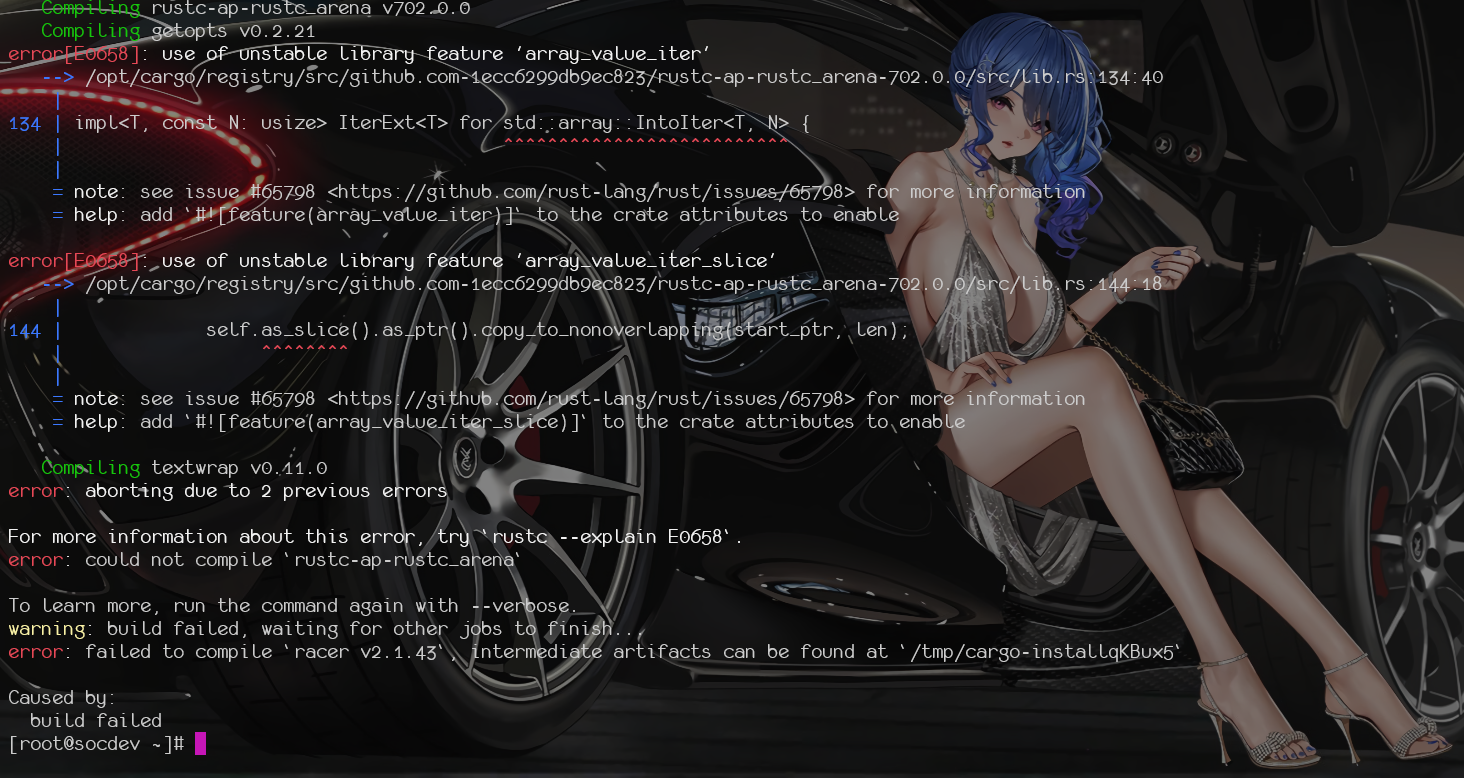
\includegraphics[width=\linewidth]{rust_feature_error.png}
  \caption{缺少特性支持编译失败}
  \label{fig:rust_feature_error}
\end{figure}
遇到这种错误,则需要直接修改对应的类库的源代码。以上述错误为例,编译的help表示
\mintinline[breaklines=true,breakanywhere,breaksymbolleft=,breakanywheresymbolpre=,]{bash}{add `#![feature(array_value_iter_slice)]` to the crate attributes to enable},
则我们应当在对应的crate的lib.rs的头部当中,添加内容如下:
\begin{figure}[H]
  \centering
  
\includegraphics[width=\linewidth]{rust_feature_add.png}
  \caption{增加特性支持}
  \label{fig:rust_feature_add}
\end{figure}
